\documentclass[a4paper, UKenglish, 11pt]{uiomaster}
\usepackage{lipsum}
\usepackage[subpreambles=true]{standalone}
\usepackage{graphicx}

\begin{document}

\chapter{Electroencephalograpy}
Electroencephalography (EEG) is a recording of the electrical activity of the cerebral cortex, representing a vital tool that has significantly contributed to our understanding of neuron interactions and the brain's organizational complexity. As one of the most widely used non-invasive techniques in neuroscience and clinical practice, EEG has played a pivotal role in studying brain activity during various cognitive processes, as well as in diagnosing diseases and estimating functional connectivity.

The roots of EEG trace back to the groundbreaking work of Hans Berger, who recorded the first human brainwave in 1924, marking the beginning of a new era in neuroscience research \cite{wiki:electroencephalography}. Since then, EEG has become an indispensable method, providing valuable insights into brain dynamics and functioning. EEG is a valuable tool that can be used to detect abnormalities in specific areas of the brain, aiding in the diagnosis of various brain disorders, including epilepsy, Alzheimer's disease, and brain tumors. By identifying distinct patterns of brain activity associated with these conditions, EEG has become an essential tool for early detection, differential diagnosis, and treatment planning.

In this chapter, our primary objectives are to explore the physiological basis of the EEG technique, shed light on the concept of the inverse problem in EEG, and introduce the use of head models to simulate realistic EEG measurements. Understanding the foundations of EEG and its methodologies will lay the groundwork when we further in this thesis will investigate the possibilities of using simulated EEG measurements to train a neural network for the purpose of localizing the sources generating these signals.

\section{The Physiological basis of the EEG}

Electroencephalography (EEG) is a technique that utilizes small metal disks known as electrodes, placed on the scalp, to detect the electrical charges resulting from the activity of brain cells. The EEG recording electrodes are typically connected to individual wires, which in turn are linked to channel connectors leading to a differential amplifier bank. An illustration of the typical EEG measurement setup is depicted in Figure \ref{fig:EEG}. By measuring the electrical potentials of cortical neuronal dendrites near the brain's surface, EEG provides valuable insights into brain function.

\begin{figure}[!htb]
    \centering
    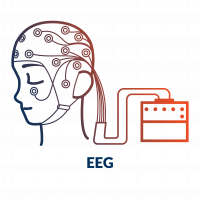
\includegraphics[width=0.6\linewidth]{figures/EEG.png}
    \caption{Illustration of the EEG method.}
    \label{fig:EEG}
\end{figure}


When a single pyramidal cell is stimulated and reaches its threshold, it generates an action potential. During this process, the synapse receives an excitatory signal, leading to a post-synaptic potential where positively charged ions enter the cell. As a result, a relatively negative charge is induced in the nearby extracellular space, which refers to the fluid-filled space surrounding the neuron. As the action potential travels down the dendrite, it eventually exits the cell membrane at locations further away from the synapse, and these locations are referred to as the "source." Consequently, an outward flow of positive charge prevails, leading to a relatively positive charge in the extracellular space. This spatial configuration creates an external dipole, with a relatively negative charge at the distant part of the dendrite and a positive charge closer to the cell body \cite{bromfield2006introduction}.

Since the electrical potential generated by an individual neuron is far too small to be picked up by the recording electrodes, the EEG measurements primarily reflect the summation of synchronous activity from thousands of pyramidal neurons with similar spatial orientation. Neurons with different geometric alignments cannot be measured as their ions do not align in a way that creates detectable waves. Due to the voltage field gradients decreasing with the square of the distance, detecting activity from deep sources in the brain is more challenging compared to currents closer to the skull \cite{bromfield2006introduction}.


The EEG is typically described in terms of rhythmic activity and transients, which are divided into frequency bands. Frequency bands are often extracted using spectral methods, and most of the cerebral signals observed in the scalp EEG fall within the range of 1–20 Hz. Abnormal activity can broadly be classified into epileptiform and non-epileptiform activity. Epileptiform activity is characteristic of people with epilepsy and includes spikes, sharp waves, and spike-wave complexes. In this context, spikes refer to hypersynchronized bursts from a sufficient number of neurons, arising from high-frequency bursts of action potentials. Generalized epileptiform discharges often exhibit an anterior maximum, seen synchronously throughout the entire brain, strongly suggestive of a generalized epilepsy \cite{bromfield2006introduction}.

Detecting and localizing abnormal electrical patterns in EEG represents a captivating research pursuit. One of the fundamental aspects in this field is the "EEG inverse problem," which aims to ascertain the spatial distribution of brain activity using potential measures acquired from scalp EEG recordings. In the upcoming section, we will explore the concept of the EEG inverse problem in greater detail and examine its implications for source localization.

\section{The Inverse Problem and Source Localization}
In the field of neuroscience, the inverse problem involves inferring the underlying parameters that caused a set of eeg measured data. Unlike the forward problem, where known parameters are used to predict the resulting eeg potential, the inverse problem lacks a unique solution. This means that more than one configuration of neural sources can ecoke one and the same distribution of EEG activity on the scalp \cite{hecker2021convdip}.

The forward problem in EEG refers to the mathematical modeling of the relationship between neural current sources in the brain ant the resulting EEG measurements on the scalp, and can mathematiccaly be described as:

\begin{equation}
\Phi(t) = L \cdot J(t)
\label{eq:forward_problem}
\end{equation}

where $\Phi$ is the vector of measured EEG signals at time $t$, $J(t)$ is the vector of unknown neural current sources at time $t$, and $L$ is the lead field matric representing the relationship between recording electrodes and the neural sources. We will come back to the meaning of the lead field matrix later on in this chapter. But for now, we think of it as a ...

The inverse problem on the other hand, is concerned with estimation the neural current sources in the brain based on the measured EEG data, i.e the inverse operation of the forward problem, and thus the name. This relationship can be expressed as:

\begin{equation}
J(t) = L^{-1} \cdot \Phi(t)
\label{eq:forward_problem}
\end{equation}

where $L^{-1}$ is the inverse of the lead field matrix.

Unlike the forward problem, the inverse problem lacks a unique solution due to the ill-posed nature of the challenge, wherein multiple sets of neural current sources can give rise to the same EEG measurements. Consequently, localizing the specific neural sources responsible for generating the EEG signals becomes a challenging and statistically driven task. In order to address the complexity associated with numerous unknowns, one commonly introduces assumptions and constraints to help mitigate the issue. These assumptions can aid in narrowing down the possible solutions and facilitate a more robust and meaningful estimation of the neural sources underlying the measured EEG data.

\subsection{The Current Dipole Approximation}

To adress the challanges of the inverse problem, one is typically befefitted with using the current dipole-approximation. This approximation is based on the observation that the neurons's contribution to the extracellular potentiol $V_e$ becomes increasingly dipoler with an increasing distance.

% what is meant by volume
% find other sources than wikipedia. vegard is hot i love him
We know that electrical charges can create current multipoles, depending on coordinates and symmetry of the charge distribution \cite{wiki:multipoles}. Similarly, the combination of current sinks and sources sets up such charge multipoles. When the distance $R$ from the center of the volume to the recording point is larger that the distance from the volume center to the most peripheral source, multipole expansion can be used \cite{jackson1999classical}.

The extracellular potential $V_e(R)$ can be expressed using the multipole expansion theorem as follows:

\begin{equation}
  \phi(R) = \frac{C_{\text{monopole}}}{R} + \frac{C_{\text{dipole}}}{R^2} + \frac{C_{\text{quadrupole}}}{R^3} + \frac{C_{\text{octopole}}}{R^4} + ... .
\label{eq:extracellular_potential}
\end{equation}

where the numerators represents the contributions to the extracellular potential. The terms denoted $C_\text{monopole}$, $C_\text{dipole}$ and $C_\text{quadrupole}$ represents contributions to the extracellulat potential, $V_e$, and can in general be extremely complicated as they depend on the relationship between radial coordinates and symmetry of the current source and measurement electrode. However, multiple expansions are often beneficial as usually only the first few terms are needed in order to provide an accurate approximation of the original funtion. This also hold in our case, as the quadrupole, octople and higher-order contributions to $V_e$ decay more rapidly with distance $R$ than the dipole contibution. Assuming that we are sufficiently far away from the source distribution, all terms above the dipole contribution vanish.

Furthermore, the monopole contribution vanishes as the net sum of currents over a neuronal membrane is always zero. This means that the monopole term also vanishes, and the expression for the extracellular potential, $V_e$ is approximated by the dipole contribution alone:


\begin{equation}
\V_e(\textbf{r}) \approx \frac{C_{\text{dipole}}}{R^2} = \frac{1}{4\pi\sigma}\frac{|\textbf{p}| cos \theta}{\lvert\textbf{r}-\textbf{r}_p\rvert^2}.
\label{eq:extracellular_potential_approximation}
\end{equation}

where we have substituded for $C_\text{dipole}$ in terms of other properties. Here, $\textbf{p}$ denotes the current dipoile moment in a medium with conductivity $\sigma$. $R = |\textbf{R}| = |\textbf{r} - \textbf{r}_p|$ is the distance between the current dipole moment at $\textbf{r}_p$ and the electrode location $\textbf{r}$. Finally $\theta$ represents the angle between $\textbf{p}$ and $\textbf{R}$. This equation is known as the dipole approximation and is a precise approximation for calculating extracellular potential, given that $R$ is much larger than the dipole length $d=|\textbf{d}|$, which is most often the case in EEG studies \cite{naess2021biophysically}.

The relationship between the current dipole moment $\textbf{p}$ and a \emph{set} of neural current sources can be expressed as follows:

\begin{equation}
\textbf{p} = \Sigma^N_{n=1}I_n\textbf{r}_n
\label{eq:extracellular_potential_approximation}
\end{equation}

where $I_n$ is the axial current inside the \emph{n}-th neuron, and $r_n$ is the position vector of the \emph{n}-th neural current source.

In Figure \ref{fig:dipole_pattern}, we have provided a simulation of the extracellular potential generated by a neuron in response to a single synaptic input, where the spatial distribution of membrane current was explicitly taken into consideration. Based on the figure, it is apparent that the distribution of electric charge in the extracellular potential of the neurons surroundings exhibits distinct dipole patterns when observed from a greater distance.

\begin{figure}
    \centering
    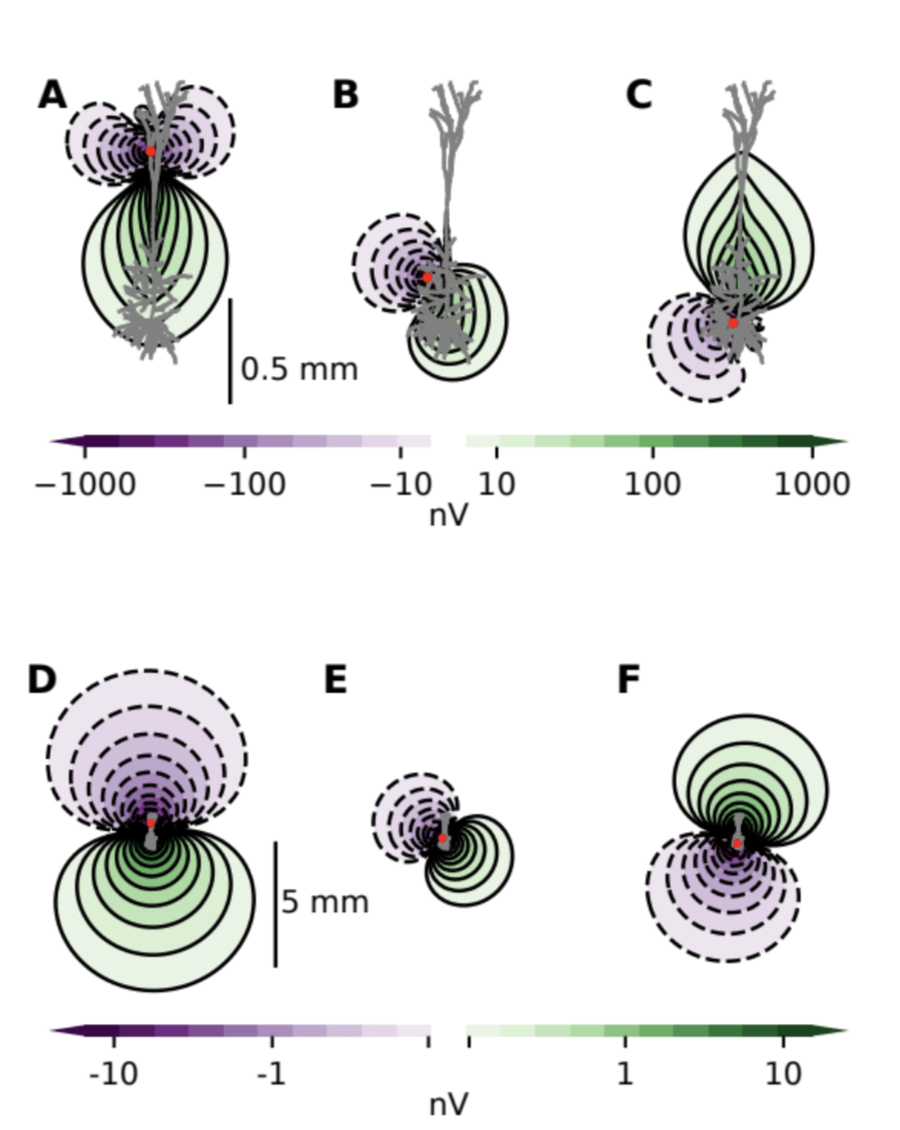
\includegraphics[width=\linewidth]{figures/dipole_pattern.png}
    \caption{Simulation of extracellulat potential showing distinct dipole pattern. The figure has been provided from my supervisiors Torbjørn Ness and Gaute Einevoll.}
    \label{fig:dipole_pattern}
\end{figure}

Solving the inverse problem can be done by the use of machine learning and neural network, whcich is the aim of this thesis. By the use of complicated Head model for the purpose of simulate biophysical realistic EEG measurement, we hope to train a neural network to localize the current dipoles geenrating the EEG signals.


% Idea : own chapter about forward modelling and the dataset right after this section ?
\section{Simulating EEG Measurements}

In order to accurately simulate EEG data and perform source localization, it is essential to utialize head models that accurately represents the conductivity distribution within the head. Head models are computational representations of the anatomical structure of the human head, including the brain, skull, cerebrospinal fluid and scalp. Head models plays an integral part in simulating how electrical current dipoles propagate through the different tissue compartments and affect the recording values at the eeg electrodes.

EEG signals are in general significantly affected by the biophysically details of the head. The conductivity of the cerebrosipinal fluid exhibits a conductivity of approximately 1.7 S/m, while the conductivity of the scull and scalp is approximately 0.01 S/m and 0.5 S/m, respectively. These conductivity variations highlight the need for more comprehensive and realistic models of the head that takes into account such conductivity variations. In addition to acount for the variations in conductivity across different regions of the head, head models also takes into account that the EEG signal from a neuronal population will depend on whether the population is located in a \emph{sulcus} or a \emph{gyrus} \cite{naess2021biophysically}. Said with other words, by utializing biophysical detailed head models, it gets taken into account the impact of various tissues on the distribution of extracellular potential, meaning one can provide more accurate simulation of EEG signal, which in turn will give more accurate solutions when solving the EEG inverse problem.

\subsection{The New York Head}
The New York Head (NYH) model is a highly detailed computer model of the human head, specifically designed for simulating the electrical activity of the brain, with a primary focus on EEG source localization. Developed by the Biomedical Engineering Department in New York, this model is based on high-resolution anatomical MRI data from 152 adult heads, enabling the segmentation of six distinct tissue types in the head: scalp, skull, cerebrospinal fluid, gray matter, white matter, and air cavities. Its high level of detail and accuracy makes it an excellent tool for simulating and comprehending brain activity in a realistic manner.

By providing a three-dimensional representation of the head and brain, along with precise information on the geometry and electrical properties of the different tissues and structures, the New York Head serves as a valuable resource for investigating brain functions, particularly in the context of EEG measurements and source localization.

For EEG simulations, the NYH model is solved for 231 specific positions representing recording electrodes on the scalp. To predict the EEG signals recorded at different scalp locations, the model utilizes a mathematical representation called the "lead field matrix." This matrix captures the relationship between the electrical activity in the brain and the electrical potentials recorded on the scalp.

The lead field matrix is essential for linking brain current density to the EEG signals recorded on the scalp. It relies on the reciprocity theorem, which connects brain current caused by an injected current between stimulating electrodes to the potentials picked up by recording electrodes. Specifically, for a fixed pair of stimulating electrodes, the lead field vectors are calculated throughout the head to determine the orientation of the dipole source that generates the largest potential difference between the electrodes. Represented by the symbol $\boldsymbol{L}$, the lead field matrix then establishes the relationship between the brain's current dipole moment and the resulting EEG signals. Mathematically, the lead field matrix $\boldsymbol{L}$ is given by:

\begin{equation}
L = \frac{E}{I},
\label{eq:R2}
\end{equation}

where $I$ represents the injected current at the electrode locations, and $E$ corresponds to the resulting electric field in the brain \cite{naess2021biophysically}. This leads to the precise connection between a current dipole moment $p$ in the brain and the resulting EEG signals $\Phi$:

\begin{equation}
\Phi = L \cdot p,
\label{eq:EEG_signal}
\end{equation}

In practical terms, when an injected current of 1 mA flows through the brain, it generates an electric potential $E$ measured in V/m. Thus, a current dipole moment $\textbf{p}$ in the unit of mAm results in EEG signals measured in the unit of V.

For further comprehensive details about the New York Head model, we refer readers to the article: https://www.parralab.org/nyhead/HauHuaPar-embc-2015.pdf.


\subsection{LFPy}


The New York Head model has been incorporated in the Python module LFPy, which provides classes for calculation of extracellular potentials from multicomparment neuron models. These tools will be utialized in this thesis. For more information read: \url{https://lfpy.readthedocs.io/en/latest/readme.html#summary}

The model utilizes the software tool LFPy, which is a Python module for calculation of extracellular potentials from multicompartment neuron models. This model takes into account that electrical potentials are effected by the geometries and conductivities of various parts of the head.

\subsection{Method}
For the purpose of ... we utialize the LFPy module and the incorporated Ney York Head.


In order to understand the underlaying mechanims of the brain and corresponding EEG recordings, biophysically detailed tools are essential. By accurately simulating EEG data,  non-linear optimization algorithms such as machine learning algortihms and neural networks can be utialized for solving the EEG inverse problem.



In order to understand the underlaying mechanims of the brain and corresponding EEG recordings, biophysically detailed tools are essential. By accurately simulating EEG data,  non-linear optimization algorithms such as machine learning algortihms and neural networks can be utialized for solving the EEG inverse problem.

% Give code example ?



% Need sources and to be rewritten


%(Do I understand this? Note: Can write much more about this. page 288.)


%\section{The New York Head Model}
% The signals received from EEG are known to originate from cortical neural activity, which are often described by using current dipoles. It is therefor reasonable to implement current dipoles in the brain for when generating a biophysical modeling of EEG signals. The brain model used in this thesis is called the New York Head model, and is based on high-resolution anatomical MRI-data from 152 adult heads. The model utilizes the software tool LFPy, which is a Python module for calculation of extracellular potentials from multicompartment neuron models. This model takes into account that electrical potentials are effected by the geometries and conductivities of various parts of the head.
%
% The cortex matrix consists of 74382 points, which refer to the number of possible positions of the dipole moment in the cortex. When generating our data set, we will for each sample randomly pick the position of the dipole moment, such that one sample corresponds to one patient. In our head model we are considering 231 electrodes uniformly distributed across the cortex, meaning that each EEG sample will consist of this many signals for each time step. However, we are not interested in the time evolution of the signals as this does not affect nor say anything about the position of the dipole moment, and we therefor simply pick out the EEG signals for when $t$ = 0 (note that the choice of time step could have been randomly picked). Our final design matrix will then consist of 1000 rows, corresponding to each patient, and 231 columns also refereed to as features, representing the signal of each electrode. The final output we are trying to predict is then the one dimensional vector with length 1000, where each element consists of the x-, y- and z- position of the dipole moment. An example of how the input EEG signals may look like is given in appendix A, where we also have marked the dipole moment with a yellow star.






%Imagining a small part of the cortex, all of these cells will have dendrites pointing upwards in the same direction (lets say the z-direction). Due to rotational symmetry around the z-axis, the contributions in the x- and y-direction will cancel. This is illustrated in Figure \ref{fig:EP}. What we see is that the extracellular potential is configured in all sorts of weird ways (A-C) when there is only one synaptic input, while the extracellular potential reminds more of a dipole when we have multiple synaptic inputs (D-F). We can therefore argue that the total contribution to the extracellular potential can be modelled as a dipole in the z -direction for the case where we have multiple synaptic inputs. Hence, for each dipole moment in our simulations, we assume multiple synaptic inputs, and make sure to rotate the positions of the dipoles such that it is orientated along the depth of the cortex.

%\begin{figure}
%    \centering
%    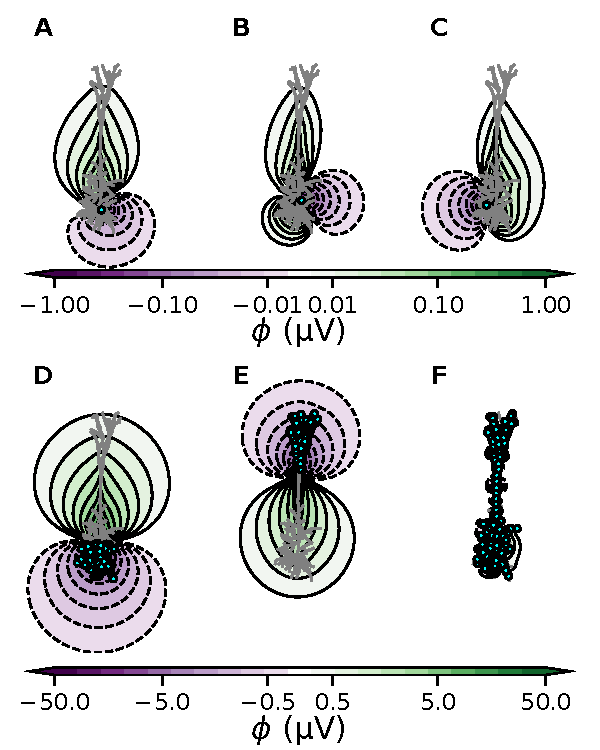
\includegraphics[width=\linewidth]{figures/fig_chosen_dipoles.pdf}
%    \caption{Extracellular potential from lonely synaptic input (A-C) and extracellular potential from multiple synaptic inputs (D-F).}
%    \label{fig:EP}
%\end{figure}








% % In EEG recordings, the current dipole approximation pyramidal cells ...
% % One approach is to assume that the EEG singals are generated of many synpatic inputs to the pyramidal neurons in cortex. Imaging a small part of the cortex, this part will be full of pyramidal cells with apikal-dendrites, that all points upwards in the same direction - we define this as the local z-direction. Due to rotational symmetry around the z-axis, the x- and y-components of the dipol will cancel, and we are left with a dipol oriented along the z-axis. With other words one assume that the source of a signal, measured with the EEG, can be modeled by a single, or sometimes, a few dipoles.
%
%
%
% \section{Forward modeling of EEG signals}
% To better understand the complexities of the inverse problem and the nuances of source localization in EEG, it is helpful to gain a deeper comprehensionin of forward modeling, involving the simulation of electrical activity of the brain as it would be measured by electrodes on the scalp.
%
% As explained in chapter 1, neural activity generates electric currents in the brain, which in turn create electromagnetic fields. In order to calculate extracellular electric potentials, one can envision the head as a 3D volume conductior, and combine Maxwell's equations with the current conservation law. We then obtain the Poisson equation for computing extracellular potentials:
%
% \begin{equation}
%   \nabla \cdot \textbf{J} = \nabla \cdot \left(\sigma \nabla \phi \right)
% \label{eq:Poisson}
% \end{equation}
%
% where \textbf{J} is the electric current density in extracellular space, $\sigma$ is the extracellular conductivity and $\phi$ is the extracellular electric potential \cite{naess2021biophysically}. For simple, symetric head models, the Poisson equation can naturally be solved analytically. However, as for the New York Head which is a complex model that we will be utialize in this thesis, we will be using the numerical method known as Finite Element Method (FEM) when solve the quation.
%
%
% To accurately calculate the extracellular potential(s), $\phi$, a well-established two-step forward-modeling approach is used. In the first step, a multicompartmental model is utialized, which takes into account the intricate details of neuron morphologies to determine the transmembrane currents, $I_n$. In the second step, equation \ref{eq:Poisson} is solved, under the assumptions that the extracellular medium acts as a volume conductor with the following properties:
%
% \begin{itemize}
%     \item infinitely large
%     \item linear
%     \item ohmic
%     \item isptropic
%     \item homogeneous
%     \item frequency-independent
% \end{itemize}
%
% The origin of extracellur potentials is spatially distributed membrane currents, entering and escaping the extracellular medium. These currents can be understood as current sources and sinks, and give the extracellular potential, $\phi$ at the electrode location $\textbf{r}$:
%
% \begin{equation}
%   \phi(\textbf{r}) = \frac{1}{4\pi\sigma}\sum^{N}_{n=1}\frac{I_n}{|\textbf{r}-\textbf{r}_n|}
% \label{eq:extracellular_potential}
% \end{equation}
%
% where $\textbf{r}_n$ is the location of the tranmembrane current $I_n$, $N$ is the number fof transmembrane currents and $\sigma$ is the extracellular conductivity \cite{naess2021biophysically}.
%
% \section{Multicompartmental modeling}
% The potential over the membrane, $V_m$, in long neurons with multi-branched dendrites varies depending on whether the potential is measured in the soma or at the tip of a sital denrite \cite{naess2021biophysically}. Multicompartmental (MC) models are models that account for this spatial variabilty in $V_m$. In such models, the neural morphology commonly is represented as isopotential cylindrical compartmens, with lengths and diameters derived from reconstructed morphologies, connected with resistors \cite{sterratt2011principles}. Single values of $V_m$ can then be computed for each individual compartment, as depiced in Figure \ref{fig:MC_models}.
%
% %TODO:
% % Fix figure text and sources
% \begin{figure}[!htb]
%     \centering
%     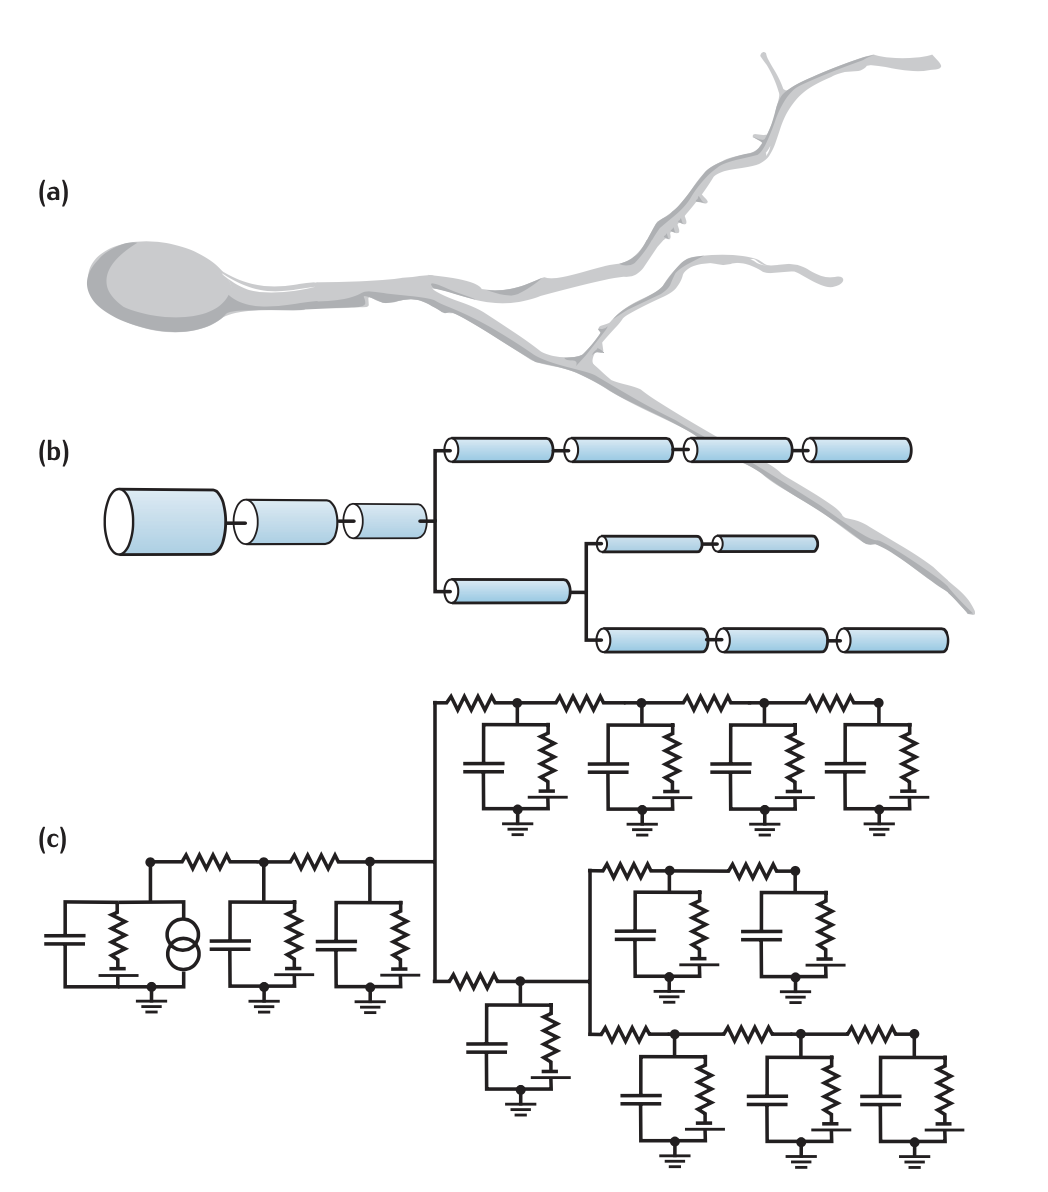
\includegraphics[width=\linewidth]{figures/MC_models.png}
%     \caption{A diagram of the development of a multi-compartmental model.
% (a) The cell morphology is represented by (b) a set of connected cylinders. An electrical circuit consisting of (c) interconnected RC circuits is then built from the geometrical properties of the cylinders, together with the membrane properties of the cell.}
%     \label{fig:MC_models}
% \end{figure}
%
% The fundamental equation for MC models is given as:
% \begin{equation}
%   c_m\frac{dV_{m,n}}{dt} = - i_{L,n} - \sum_w i_{w,n} - \frac{I_{\text{syn},n}}{\pi dL} + \frac{I_{\text{ext},n}}{\pi dL} \frac{d}{4r_a}\left( \frac{V_{m,n+1} - V_{m,n}}{L^2} - \frac{V_{m,n} - V_{m,n-1}}{L^2} \right )
% \label{eq:MC}
% \end{equation}
%
% where ....
%
% This equation (\ref{eq:MC}) assumes that a compartment $n$ has two neighbors - one at $n - 1$ and the second at $n - 2$. However, when considering the endpoint compartments, this clearly will not be true. A commonly used boundry condition, is the sealed-end condition, where no axial currents leave at the cable endpoints. With other words this means that $I_{0,1} = 0$ in one end of the cable, and $I_{N,N+1} = 0$ in the other end. For the cable endpoints, we are then left with the following expressions:
%
% \begin{equation}
%   c_m\frac{dV_{m,1}}{dt} = - i_{L,1} - \sum_w i_{w,1} - \frac{I_{\text{syn},1}}{\pi dL} + \frac{I_{\text{ext},1}}{\pi dL} \frac{d}{4r_a}\left( \frac{V_{m,2} - V_{m,1}}{L^2} \right )
% \label{eq:MC_end1}
% \end{equation}
%
% and
%
% \begin{equation}
%   c_m\frac{dV_{m,N}}{dt} = - i_{L,N} - \sum_w i_{w,N} - \frac{I_{\text{syn},N}}{\pi dL} + \frac{I_{\text{ext},n}}{\pi dL} \frac{d}{4r_a}\left( \frac{V_{m,N} - V_{m,N-1}}{L^2} \right )
% \label{eq:MC_end2}
% \end{equation}
%
% %TODO
% % Some equation for the
%
% \section{Volume conductors}
% As mentioned above, we can use volume conductor (VC) theory to predict the resulting extracellular potential $V_e$ at any given point in space, given that the distribution of neuronal membrane currents is known.
%
% % What should I include here?
%
% \section{Head Models}
% The analytical formula presented in Equation \ref{eq:extracellular_potential_approximation} was dereived based on the assumption of a constant tissue conductivity, denoted as $\sigma$. However, because the EEG signals is measured outside the head, it is affected by the different conductivities og the brain, verebrospinal fluid (CSF), skull and scalp. Depending on problem, it may be important to keep in mind that EEG signals, in general, are significantly affected by biophysically details of the head. For instance, the conductivity of the cerebrosipinal fluid exhibits a conductivity of approximately 1.7 S/m, while the conductivity of the scull and scalp is approximately 0.01 S/m and 0.5 S/m, respectively. These conductivity variations highlight the need for more comprehensive and realistic models of the head, known as head models, which take into account such conductivity variations. In addition to acount for the variations in conductivity across different regions of the head, head models also takes into account that the EEG signal from a neuronal population will depend on whether the population is located in a \emph{sulcus} or a \emph{gyrus} \cite{naess2021biophysically}. Said with other words, by integrating biophysical details into models, a deeper understanding emerges regarding the impact of various tissues on the distribution of extracellular potential, which in turn, can lead to improvements in the accuracy of EEG signal analysis.
%
%
% \subsection{The New York Head}
% A central problem for EEG is to relate scalp data to brain \emph{current sources} (Electric Fields of the Brain: The Neurophysics of EEG)....
%
% Especially important for electrode locations outside of the brain, such as EEG, is the knowledge about how the electrical potentials will be affected by the geometries and conductivites of the various parts of the head \cite{naess2021biophysically}. A model that takes these detailes into account is the New York Head Model. The model is based on anatomical and electrical characteristics of 152 adult human brains and is solved for 231 electrode locations.
%
% The New York Head Model is a computer model of the human head used to simulate the electrical activity of the brain. It was created by the Electrical Geodesics Incorporated (EGI) in 2004, and is based on the anatomical and electrical characteristics of the head of a typical adult human. The model consists of a three-dimensional (3D) representation of the head and brain, with detailed information on the geometry and electrical properties of the different tissues and structures within the head. The model includes the scalp, skull, cerebrospinal fluid, gray matter, and white matter. The electrical properties of each of these tissues, such as conductivity and permittivity, are also included in the model.
% % Need sources and to be rewritten
%
% The model was developed to be used for, and improve the accuracy of EEG source localization \cite{huang2016new}. To generate predictions of the EEG signals recorded from different scalp locations in response to a given set of source currents, the New York head model uses the lead field matrix (SOURCE), which is a mathematical representation of the relationship between the electrical activity in the brain and the electrical potentials recorded on the scalp.
%
% \begin{figure}
%   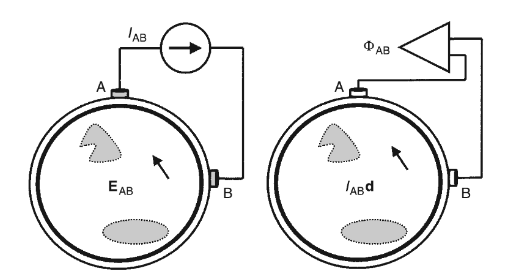
\includegraphics[width=\linewidth]{figures/lead_fields.png}
%   \caption{A caption here is needed.}
%   \label{fig:lead_field}
% \end{figure}
%
% The lead field matrix is constructed by taking advantage of the reciprocity theorem that states that knowledge of the current density through a volume conducter caused by an injection of current between two stimulating electrodes completely specifies how those same recording electrodes pick up potentials caused by dipole sources in the volume conducter. If one suppose that a pair of stimulating electrodes is placed at locations A and B on the scalp as provided in figure \ref{fig:lead_field}, an external current source will cause current to flow from electrode B through the brain, and all the way to electrode A. However, due to the geometry, inhomogeneity, and ansisotropy of the head, the current density will vary with location. The amount of current that pass through the brain depends, to a great extent, on the location of the electordes. In general, the brain currents will decrease with decreasing distance between electrodes. Thus, for a fixed pair of electrodes, the lead field vectors can be calculated as a function of position throughout a volume conducter. At each location, the orientation of the lead field vector $L_{AB}$ is the orientation of the dipole source that produces the largest potential difference between the electrodes. The lead field matrix, $\boldsymbol{L}$ is given as:
%
% \begin{equation}
% L = \frac{E}{I},
% \label{eq:R2}
% \end{equation}
%
% where $I$ is the injected current at the electode locations and $E$ is the resulting electric field in the brain \cite{naess2021biophysically}. Moreover, the precise link between a current dipole moment $p$ in the brain and the resulting EEG signals $\Phi$ is then related to the lead field matrix as follows:
%
% \begin{equation}
% \Phi_{AB} = L_{AB} \cdot p,
% \label{eq:EEG_signal}
% \end{equation}
%
% Here, an injected current $I$ of 1 mA gives an electric potential $E$ in V/m, meaning that a current dipole moment $\textbf{p}$ in the unit of mAm gives EEG signals in the unit of V.
%
% %(Do I understand this? Note: Can write much more about this. page 288.)
%
% The New York Head model has been incorporated in the Python module LFPy, which provides classes for calculation of extracellular potentials from multicomparment neuron models. These tools will be utialized in this thesis. For more information read: \url{https://lfpy.readthedocs.io/en/latest/readme.html#summary}
%
% %\section{The New York Head Model}
% The signals received from EEG are known to originate from cortical neural activity, which are often described by using current dipoles. It is therefor reasonable to implement current dipoles in the brain for when generating a biophysical modeling of EEG signals. The brain model used in this thesis is called the New York Head model, and is based on high-resolution anatomical MRI-data from 152 adult heads. The model utilizes the software tool LFPy, which is a Python module for calculation of extracellular potentials from multicompartment neuron models. This model takes into account that electrical potentials are effected by the geometries and conductivities of various parts of the head.
%
% The cortex matrix consists of 74382 points, which refer to the number of possible positions of the dipole moment in the cortex. When generating our data set, we will for each sample randomly pick the position of the dipole moment, such that one sample corresponds to one patient. In our head model we are considering 231 electrodes uniformly distributed across the cortex, meaning that each EEG sample will consist of this many signals for each time step. However, we are not interested in the time evolution of the signals as this does not affect nor say anything about the position of the dipole moment, and we therefor simply pick out the EEG signals for when $t$ = 0 (note that the choice of time step could have been randomly picked). Our final design matrix will then consist of 1000 rows, corresponding to each patient, and 231 columns also refereed to as features, representing the signal of each electrode. The final output we are trying to predict is then the one dimensional vector with length 1000, where each element consists of the x-, y- and z- position of the dipole moment. An example of how the input EEG signals may look like is given in appendix A, where we also have marked the dipole moment with a yellow star.
%
%
%
%
%
%
% %Imagining a small part of the cortex, all of these cells will have dendrites pointing upwards in the same direction (lets say the z-direction). Due to rotational symmetry around the z-axis, the contributions in the x- and y-direction will cancel. This is illustrated in Figure \ref{fig:EP}. What we see is that the extracellular potential is configured in all sorts of weird ways (A-C) when there is only one synaptic input, while the extracellular potential reminds more of a dipole when we have multiple synaptic inputs (D-F). We can therefore argue that the total contribution to the extracellular potential can be modelled as a dipole in the z -direction for the case where we have multiple synaptic inputs. Hence, for each dipole moment in our simulations, we assume multiple synaptic inputs, and make sure to rotate the positions of the dipoles such that it is orientated along the depth of the cortex.
%
% %\begin{figure}
% %    \centering
% %    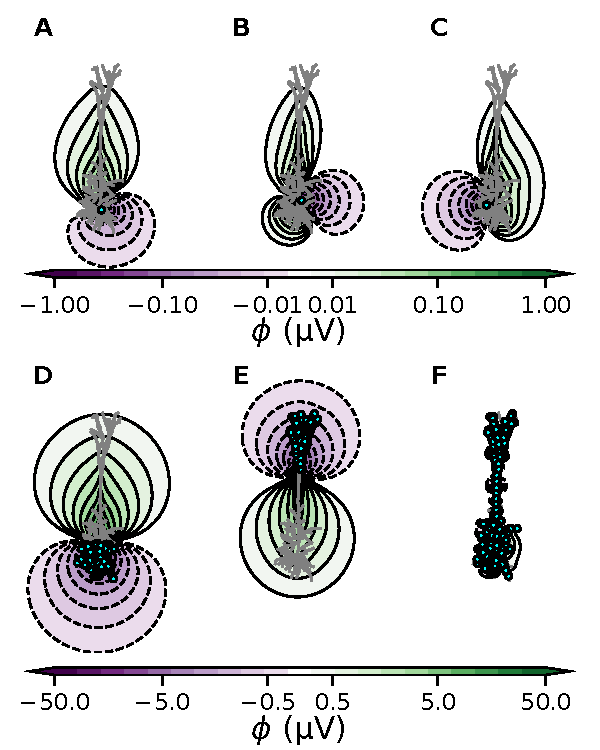
\includegraphics[width=\linewidth]{figures/fig_chosen_dipoles.pdf}
% %    \caption{Extracellular potential from lonely synaptic input (A-C) and extracellular potential from multiple synaptic inputs (D-F).}
% %    \label{fig:EP}
% %\end{figure}
%
%
% \section{The Inverse Problem and Source Localization}
%
% % To solve the inverse EEG problem, various algorithms and methods have been developed, such as Minimum Norm Estimates (MNE), Low Resolution Electromagnetic Tomography (LORETA), and Dynamic Imaging of Coherent Sources (DICS). MACHINE LEARNIG....
%
% % The inverse EEG problem is the problem of determining the sources of electrical activity within the brain that give rise to the measured EEG signal. The EEG signal is a recording of the electrical activity of the brain, which is measured at the surface of the scalp. However, the electrical activity that gives rise to the EEG signal is generated by a large number of sources within the brain, and it is not possible to determine the location or number of these sources just by looking at the EEG signal alone. Therefore, the inverse EEG problem is the problem of determining the sources of the EEG signal based on the measurement of the signal itself.
%
% % To solve the inverse EEG problem, various algorithms and methods have been developed, such as Minimum Norm Estimates (MNE), Low Resolution Electromagnetic Tomography (LORETA), and Dynamic Imaging of Coherent Sources (DICS).
%
% % However, the problem remains very challenging, as the EEG signal measured at the scalp is the result of a complex and unknown combination of sources, the brain anatomy itself and the volume conductor contribute to the complexity of the problem.
%
% % As of now, there is not yet a definitive solution for the Inverse EEG problem and the area is still active research topic.












%
% \subsection{The New York Head}
%
% The New York Head (NYH) model is a highly detailed computer model of the human head, specifically designed for simulating the electrical activity of the brain, with a primary focus on EEG source localization. Developed by the Biomedical Engineering Department in New York, this model is based on high-resolution anatomical MRI data from 152 adult heads, enabling the segmentation of six distinct tissue types in the head: scalp, skull, cerebrospinal fluid, gray matter, white matter, and air cavities. Its high level of detail and accuracy makes it an excellent tool for simulating and comprehending brain activity in a realistic manner. By providing a three-dimensional representation of the head and brain, along with precise information on the geometry and electrical properties of the different tissues and structures, the New York Head serves as a valuable resource for investigating brain functions, particularly in the context of EEG measurements and source localization.
%
% The model is solved for 231 electrode locations, meaning that it is able to generate predictions of the EEG signals corresponding to 231 specific positions for recording electrodes on the sclap. To generate predictions of the EEG signals recorded from different scalp locations in response to a given set of source currents, the New York head model uses the lead field matrix , which is a mathematical representation of the relationship between the electrical activity in the brain and the electrical potentials recorded on the scalp.
%
% \begin{figure}
%   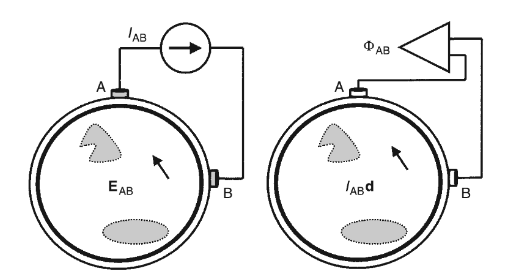
\includegraphics[width=\linewidth]{figures/lead_fields.png}
%   \caption{A caption here is needed.}
%   \label{fig:lead_field}
% \end{figure}
%
% The lead field matrix is constructed by taking advantage of the reciprocity theorem that states that knowledge of the current density through a volume conducter caused by an injection of current between two stimulating electrodes completely specifies how those same recording electrodes pick up potentials caused by dipole sources in the volume conducter. If one suppose that a pair of stimulating electrodes is placed at locations A and B on the scalp as provided in figure \ref{fig:lead_field}, an external current source will cause current to flow from electrode B through the brain, and all the way to electrode A. However, due to the geometry, inhomogeneity, and ansisotropy of the head, the current density will vary with location. The amount of current that pass through the brain depends, to a great extent, on the location of the electordes. In general, the brain currents will decrease with decreasing distance between electrodes. Thus, for a fixed pair of electrodes, the lead field vectors can be calculated as a function of position throughout a volume conducter. At each location, the orientation of the lead field vector $L_{AB}$ is the orientation of the dipole source that produces the largest potential difference between the electrodes. The lead field matrix, $\boldsymbol{L}$ is given as:
%
% \begin{equation}
% L = \frac{E}{I},
% \label{eq:R2}
% \end{equation}
%
% where $I$ is the injected current at the electode locations and $E$ is the resulting electric field in the brain \cite{naess2021biophysically}. Moreover, the precise link between a current dipole moment $p$ in the brain and the resulting EEG signals $\Phi$ is then related to the lead field matrix as follows:
%
% \begin{equation}
% \Phi_{AB} = L_{AB} \cdot p,
% \label{eq:EEG_signal}
% \end{equation}
%
% Here, an injected current $I$ of 1 mA gives an electric potential $E$ in V/m, meaning that a current dipole moment $\textbf{p}$ in the unit of mAm gives EEG signals in the unit of V.



\end{document}